
\chapter{Introduction}

The Web is an ever growing institution\textit{(entity)}, in all aspects that it covers.
The number of information and functionality providers for the Web is growing in the whole spectrum from bigger computing centers down to smaller devices.
Computing centers, growing in size and quantity, allow for massive amounts of data to be stored and accessed, but they also enable the construction and accessibility of more complex functionalities.
Ever smaller devices provide informations and functionalities to the Web, through their quickly increasing number.
Many of them are even providing access to the Web itself and thus leverage the effect of the growing Web.
For example mobile phones can act as a hotspot to grant Web access to others through \textrm{WiFi}.
\index{Web of Things}
All the smart \textrm{Things} with access to the Web start to form the \textrm{Web of Things}~\cite{Guinard2011WoT}.
This can be every\textrm{Thing} from a temperature sensor to all electronical devices within a house.
These \textrm{Things} do not only provide sensor data but they can also be easily controlled through the Web.

Confronted with this rapid growth of the Web, an increasing number of human beings is exposed to it in their daily life and they get literally flooded with data and possibilities to govern them.
Even though they have access to all these services in the Web, they often lack the knowledge, necessary time or right approach to weild them.
Users need ways to get appropriate informations, in the right moment, automatically and in a condensed matter that suits them best.
They have to be able to automate tedious tasks, e.g. detecting relevant changes in information resources and react on behalf of such changes.
% More concrete example?
This requires the identification of and filtering for user-specific information, appropriate timing, assembly and preprocessing of different information resources and finally the forwarding of outcomes to services in the web. 

Users don't want to be bound to a specific platform, but want to use the best service the Web has to offer them for their work.
Some services in the web might have means to spread their data to other pre-defined services, but they are often mere copy/paste task.
Therefore users end up mashing up informations or functionalities from different locations within the Web periodically by hand.
This leads to redundantly executed procedures with only little parametrization.
It is also likely that the completion of such a task suffers from a latency due to the deferred detection of the initialization or the user just not being able to execute the work at that time.

\begin{figure}[!ht]
  \centering
  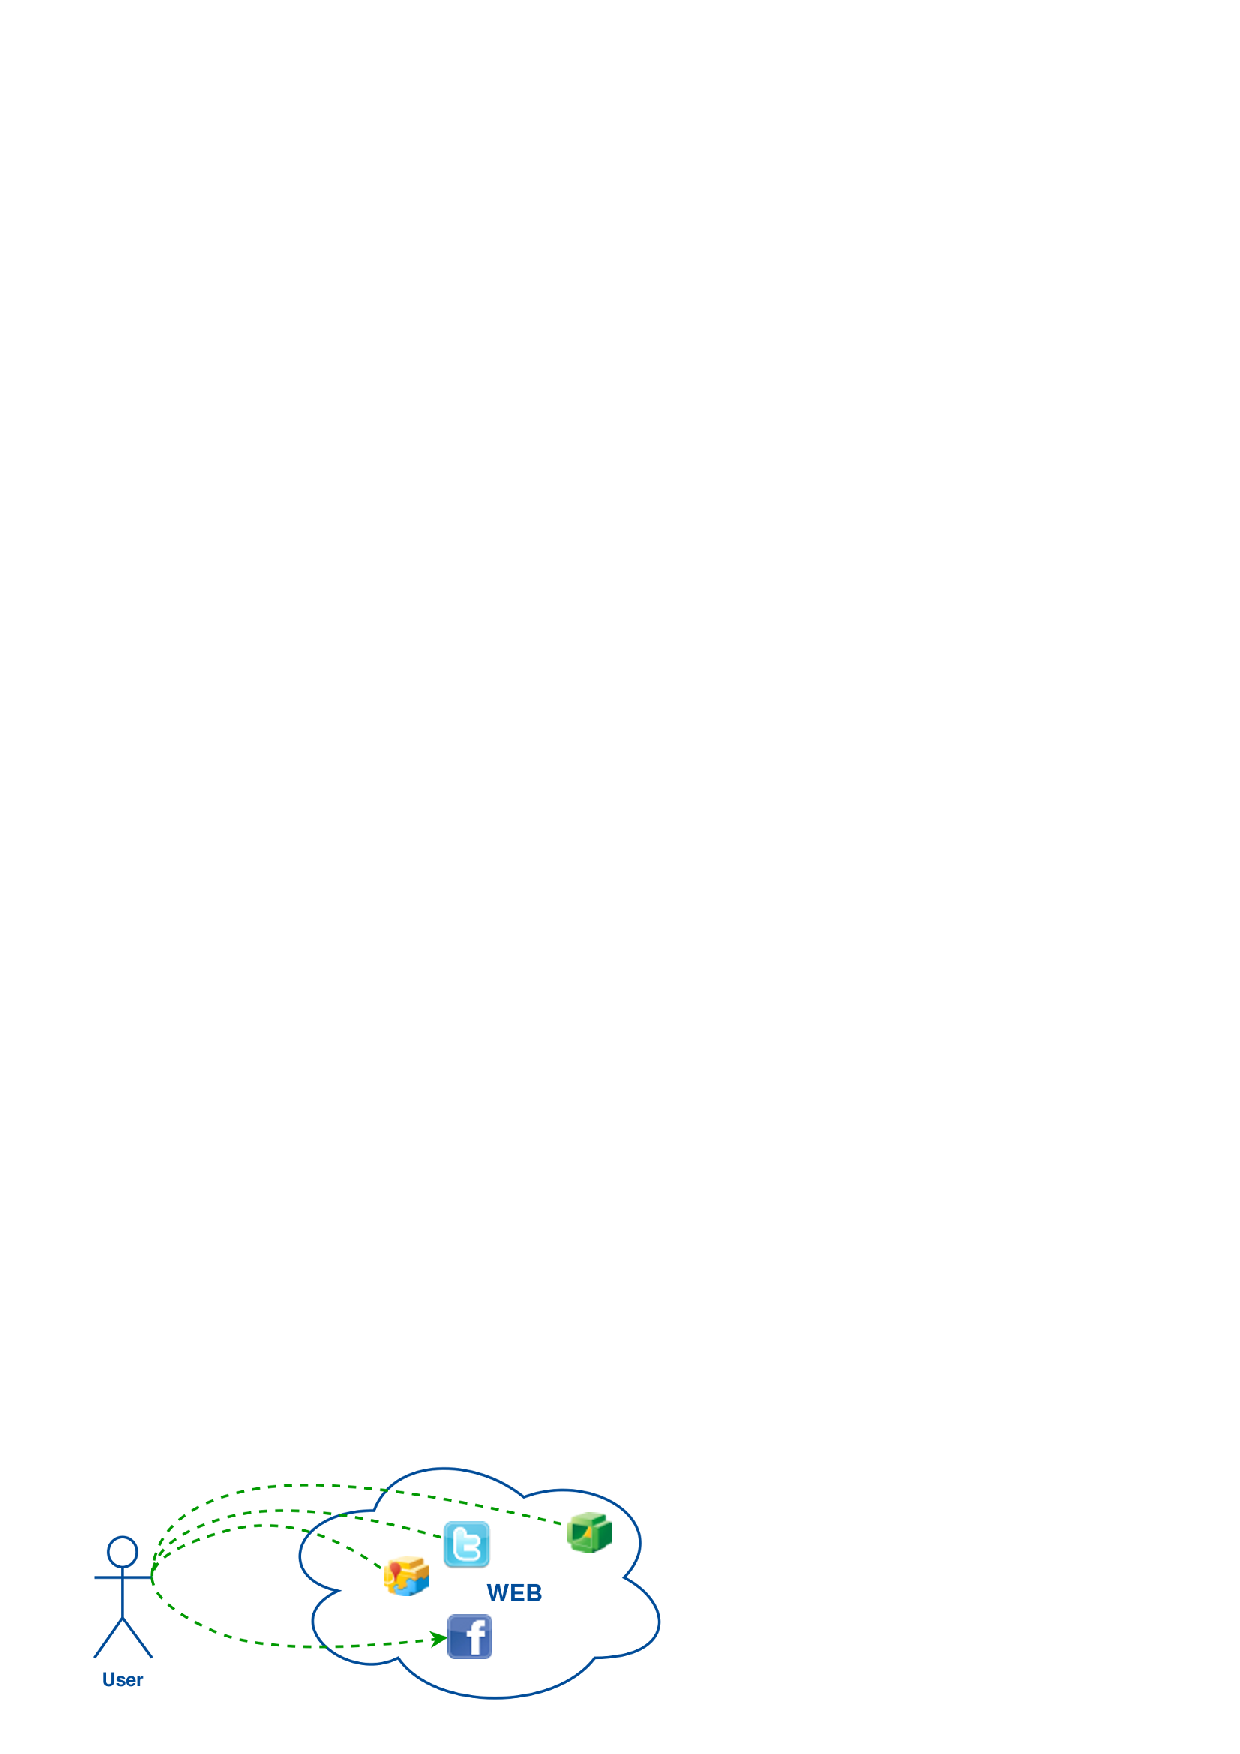
\includegraphics[width=0.7\textwidth]{figures/UsersWeildServicesInTheWeb}
  \caption{Users mashup the Web's Information and Data}
  \label{fig:UsersWeildServicesInTheWeb}
\end{figure}

A big part of the informations, that become available to the users, are short-lived informations corresponding to certain state changes, and therefore can be modeled as events.


Even if the Web service access gets simpler these days, the average user is not able to weild them.
The challenge to provide users with ways to handle these already simpler accessible services, called Web API's has received a notable amount of attention over the last few years.

We claim the whole Web as our information space in order to impose reactivity to it.
% We envision an event-driven conceptual model that allows to impose reactivity on the Web.
% Through such a model the Web should become programmable
% user-centric reactions to allow a personalization of the information flood


% Retain manageable interactions between cloud applications
% reactive rules together with cloud applications have the potential to overcome limitations 
% Current approaches concentrate on data flow rather than on event flow. which is mere data copy and spreading than reactivity
% Large systems such as \emph{RuleResponder} weave stubs or proxies of existing service into a message oriented middleware (MoM). We envision the web itself is used as the middleware. Through this a lightweighted and performant event-based architecture can be realized, which allows the orchestration of existing web and cloud applications.


It is a promising research field that leads towards reactivity in the Web through programmability.
Currently somebody that want's to program the Web, requires deep knowledge of the required services and their functionality.
There are a few possibilities in the Web that go towards easing the programmability of the Web, but they are either complicated to weild themselves or mere data copy or mashup tasks.
Our research in this thesis is about easing the programmability of the Web and therefore to achieve the reactive Web. 
